\documentclass[12pt,a4paper]{article} 
\usepackage{tikz}
\usepackage{float}
\usepackage{graphicx}
\usepackage{multirow}
\usepackage{setspace} 
\usepackage{graphicx}
\usepackage{times}
\pagenumbering{roman}
\usepackage{geometry}

\geometry{verbose,tmargin=2cm,bmargin=2cm,lmargin=3cm,rmargin=2cm}
\usepackage{fancyhdr} 
%\linespread{1.05} 
\usepackage{tikz}
\usetikzlibrary{arrows}
\usetikzlibrary{shapes.geometric}

\tikzstyle{kres} = [rectangle, rounded corners, minimum width=1cm, minimum height=0.5cm,text centered, draw=black]
\tikzstyle{nad} = [trapezium, trapezium left angle=60, trapezium right angle=100, minimum width=1cm, minimum height=0.5cm, text centered, draw=black]
\tikzstyle{sim} = [trapezium, trapezium left angle=60, trapezium right angle=100, minimum width=1cm, minimum height=0.5cm, text centered, draw=black]
\tikzstyle{garis} = [thick,->,>=stealth]
\usetikzlibrary{shapes,arrows}

\begin{document} % Mulai Penulisan Laporan
\onehalfspacing
\begin{titlepage}

\title{\textbf{LAPORAN PRAKTIKUM ELEKTRONIKA DASAR
\\ Motor DC }}  %Judul Laporan
%\title{\textbf{FOTOKATALISIS}}  %Judul Laporan
\author{\textbf {Dosen : Mada Sanjaya WS, Ph.D  }
\\ \textbf{Asisten Lab : Dikha Khameswara (1177030010)}
\\ \textbf{ }
\\ \textbf{Disusun Oleh :}
\\ \textbf{Muhamad Fahmi Adzkar} \textbf {(1187030024)}
\\ \textbf{Kelompok 3 :}
\\ \textbf{Hani Hikmawati} \textbf {(1187030014)}
\\ \textbf{Sri Rahayu} \textbf {(1187030036)}
\\ \textbf{Yuni Rahayu} \textbf {(1187030041)}}

\maketitle
\begin{center}
\vspace{1cm}

\includegraphics[width=4cm]{uin.png}
\vspace{1cm}

JURUSAN FISIKA\\
FAKULTAS SAINS DAN TEKNOLOGI\\
UIN SUNAN GUNUNG DJATI BANDUNG\\
2019\\
\end{center}
\end{titlepage}

\renewcommand\abstractname{Abstract} %Untuk Abstrak Bahasa Inggris
\begin{abstract}
Alhamdulillah, in this experiment we conducted an experiment for a transistor as switch 2 (automatic garden lights) and the introduction of the op-amp as a comparator. A transistor is a semiconductor device used as an amplifier, as a circuit breaker and connector (switching), voltage stabilization, signal modulation or as other functions. Transistors can function like an electric faucet, where based on the input current (BJT) or the input voltage (FET), allows a very accurate flow of electricity from the mains circuit. In general, transistors have 3 terminals, namely Base (B), Emitter (E) and Collector (C). The voltage in one terminal, for example, the Emitter can be used to regulate the current and voltage that is greater than the Basis input current, ie at the output voltage and the Collector output current.

\subparagraph{ }
\textit{Keywords:transistors, potentiometers, photoresistors, operational amplifiers, comparators}

\end{abstract}

\renewcommand\abstractname{Abstrak} %Untuk Abstrak Bahasa Indonesia
\begin{abstract}
	alhamdulillah pada percobaan kali ini kita melakukan percobaan untuk transistor sabagai saklar 2 (lampu taman otomatis) dan pengenalan op-amp sebagai komparator. Transistor adalah alat semikonduktor yang dipakai sebagai penguat, sebagai sirkuit pemutus dan penyambung (switching), stabilisasi tegangan, modulasi sinyal atau sebagai fungsi lainnya. Transistor dapat berfungsi semacam kran listrik, di mana berdasarkan arus inputnya (BJT) atau tegangan inputnya (FET), memungkinkan pengaliran listrik yang sangat akurat dari sirkuit sumber listriknya. Pada umumnya, transistor memiliki 3 terminal, yaitu Basis (B), Emitor (E) dan Kolektor (C). Tegangan yang di satu terminalnya misalnya Emitor dapat dipakai untuk mengatur arus dan tegangan yang lebih besar daripada arus input Basis, yaitu pada keluaran tegangan dan arus output Kolektor.


\subparagraph{ }
\textit{Kata Kunci:transistor, potensiometer, photoresistor,  operational amplifier, komparator}

\end{abstract}

\newpage
\section{PENDAHULUAN}
\paragraph{1.1 Latar Belakang}
\subparagraph{ }
	Dalam sebuah rangkaian listrik dikenal dengan istilah arus listrik (I), tegangan atau beda potensial (V) dan hambatan (R. Pada dasarnya sebuah rangkaian listrik terjadi ketika sebuah penghantar mampu dialiri electron bebas secara terus menerus. Aliran inilah yang disebut dengan arus. Sedangkan tegangan adalah beda potensial yang ada di antara titik rangkaian listrik tersebut. Untuk menemukan hubungan di antara istilah-istilah yang ada dalam sebuah rangkaian listrik diperlukan sebuah praktikum yang dapat membuktikannya.
\subparagraph{ }
	Dengan melakukan praktikum yang berjudul transistor sabagai saklar 2 (lampu taman otomatis) dan pengenalan op-amp sebagai komparator ini kita dapat mengetahui dan mempelajari Fungsi Transistor sebagai Saklar dan Prinsip Kerja Lampu Taman Otomatis. Selain itu materi tentang komparator ini sangat berguna untuk memahami prinsip kerja dari Rangkaian komparator khususnya yang mendalami kelistrikan. Dan juga Rangkaian Komparator ini sangat berhubungan dengan alat-alat otomatis yang terjadi disekitar kita, salah satunya Karakteristik Rangkaian Komparator Sebagai Aplikasi Dari Rangkaian OP-Amp yang sangat bermanfaat bagi kehidupan manusia.

\paragraph{1.2 Tujuan}
\subparagraph{•}
Adapun tujuan dilakukannya praktikum ini yaitu:
\begin{enumerate}
\item Memahami Fungsi Transistor sebagai Saklar.
\item Memahami Prinsip Kerja Lampu Taman Otomatis.
\item Memahami Perbedaan Fungsi Transistor PNP dan NPN.
\item Mengetahui Karakteristik Rangkaian Komparator Sebagai Aplikasi Dari Rangkaian OP-Amp.
\item Memahami Prinsip Kerja Dari Rangkaian Komparator.
\item Memahami Prinsip kerja Motor DC
\end{enumerate}


\newpage
\section{Landasan Teori}
\subsection{Dasar Teori}
\paragraph{ }
\textbf{Motor DC}
\subparagraph{ }
Motor Listrik DC atau DC Motor adalah suatu perangkat yang mengubah energi listrik menjadi energi kinetik atau gerakan (motion). Motor DC ini juga dapat disebut sebagai Motor Arus Searah. Seperti namanya, DC Motor memiliki dua terminal dan memerlukan tegangan arus searah atau DC (Direct Current) untuk dapat menggerakannya. Motor Listrik DC ini biasanya digunakan pada perangkat-perangkat Elektronik dan listrik yang menggunakan sumber listrik DC seperti Vibrator Ponsel, Kipas DC dan Bor Listrik DC.

	Motor Listrik DC atau DC Motor ini menghasilkan sejumlah putaran per menit atau biasanya dikenal dengan istilah RPM (Revolutions per minute) dan dapat dibuat berputar searah jarum jam maupun berlawanan arah jarum jam apabila polaritas listrik yang diberikan pada Motor DC tersebut dibalikan. Motor Listrik DC tersedia dalam berbagai ukuran rpm dan bentuk. Kebanyakan Motor Listrik DC memberikan kecepatan rotasi  sekitar 3000 rpm hingga 8000 rpm dengan tegangan operasional dari 1,5V hingga 24V. Apabile tegangan yang diberikan ke Motor Listrik DC lebih rendah dari tegangan operasionalnya maka akan dapat memperlambat rotasi motor DC tersebut sedangkan tegangan yang lebih tinggi dari tegangan operasional akan membuat rotasi motor DC menjadi lebih cepat. Namun ketika tegangan yang diberikan ke Motor DC tersebut turun menjadi dibawah 50 dari tegangan operasional yang ditentukan maka Motor DC tersebut tidak dapat berputar atau terhenti. Sebaliknya, jika tegangan yang diberikan ke Motor DC tersebut lebih tinggi sekitar 30 dari tegangan operasional yang ditentukan, maka motor DC tersebut akan menjadi sangat panas dan akhirnya akan menjadi rusak.
	
	Pada saat Motor listrik DC berputar tanpa beban, hanya sedikit arus listrik atau daya yang digunakannya, namun pada saat diberikan beban, jumlah arus yang digunakan akan meningkat hingga ratusan persen bahkan hingga 100 atau lebih (tergantung jenis beban yang diberikan). Oleh karena itu, produsen Motor DC biasanya akan mencantumkan Stall Current pada Motor DC. Stall Current adalah arus pada saat poros motor berhenti karena mengalami beban maksimal.



\newpage
\section{METODE PRAKTIKUM}
\subsection{Waktu dan Tempat}
\paragraph{ }
Praktikum ini dilaksanakan pada:
\\ 		Tanggal : jum'at, 25 oktober 2019
\\ 		Waktu : 07.00 WIB - Selesai
\\ 		Tempat : Advance Physics 


\subsection{Alat dan Bahan}
Alat dan bahan yang digunakan dalam praktikum ini diantaranya adalah : 
\subparagraph*{ }
\begin{tabular}{|l|l|l|}  \hline
No & Alat dan Bahan  & Jumlah  \\ \hline
1  & Projek board & 1 Buah \\ \hline
2  & perlengkapan lampu & satu set \\ \hline
3  & Relay & 1 Buah \\ \hline
4  & Buzzer & 1 buah  \\ \hline
5  & Transistor NPN BC547 & 1 Buah \\ \hline
6  & Transistor PNP BC557 & 1 Buah \\ \hline
7  & LDR & 1 Buah \\ \hline
8  & Baterai 9 volt & Secukupnya \\ \hline
9  & Kancing Baterai 3 Pin & 1 Buah \\ \hline
10 & Kabel Tunggal  & Secukupnya \\ \hline
11 & LED Warna & 1 Buah \\ \hline
12 & Resistor  & 4 Buah \\ \hline
13 & Potensiometer & 1 Buah \\ \hline
14 & Lampu 3 volt & Secukupnya \\ \hline
15 & Multimeter & Secukupnya \\ \hline
16 & Motor DC   & secukupnya \\  \hline

\end{tabular}

  
    
\subsection{Prosedur Percobaan}
\subparagraph{3.3.1 Percobaan Rangkaian Motor DC }
\subparagraph{ }
\textbf{Rangkaian Motor DC} 
	Siapkan alat dan bahan yang digunakan, Rangkaian disusun sesuai dengan gambar project board. Kemudian Lakukan pengecekan terhadap setiap komponen. Dilanjut dengan memastikan motor dc, Bila rangkaian transistor sebagai saklar telah dibuat, hubungkan output ke kontroler motor dc. Jadikan transistor sebagai saklar. Lakukan uji coba pada rangkaian motor dc. Sinari Ldr pada salah satu rangkaian transistor sebagai saklar. perhatikan, apakah robot mengikuti cahaya?, Apabila tidak mengikuti cahaya, maka pindahkan output transistor. Bila motor dc bergerak mundur, maka ubahlah polaritas motor dc. Bila motor tidak berjalan sebagaimana mestinya, maka ambil data, kemudian catat hasil percobaan di tabel dan analisis.
	
\begin{figure}
\paragraph{ }
\begin{center}
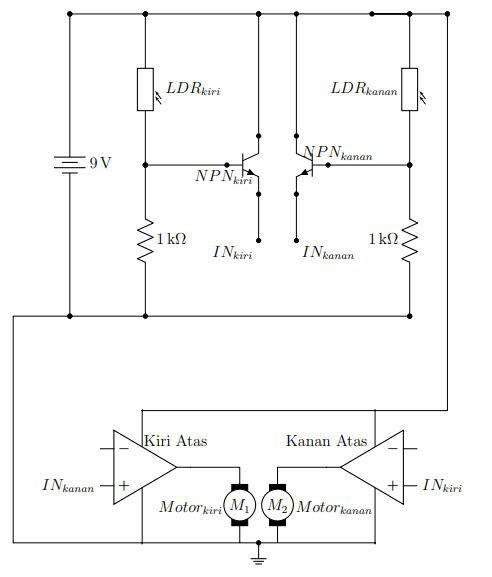
\includegraphics[width=6cm, height=12cm]{g3.png}
\end{center}
\end{figure}
\vspace{2cm}

\subsection{Diagram Alir}
\subsubsection{Percobaan Rangkaian Motor DC }
\tikzstyle{line} = [draw, -latex']
\tikzstyle{cloud} = [draw, rectangle,fill=blue!20, node distance=3cm,
    minimum height=0.7cm]
\tikzstyle{kres} = [draw, rectangle, rounded corners,fill=blue!20, node distance=3cm,
    minimum height=0.7cm]
\begin{tikzpicture}[node distance = 1.3cm, auto]
    % Place nodes
       \node [kres] (a) {Siapkan alat dan bahan yang digunakan};
       \node [cloud, below of = a , node distance = 1.5cm] (b) {Susun rangkaian sesuai dengan gambar};         
       \node [cloud, below of = b , node distance = 1.5cm] (c) {Lakukan pengecekan terhadap setiap komponen};
       \node [cloud, below of = c , node distance = 1.5cm] (d) {Memastikan motor dc};
       \node [cloud, below of = d , node distance = 1.5cm] (e) {Bila rangkaian transistor sebagai saklar telah dibuat, hubungkan output ke kontroler motor dc};        
       \node [cloud, below of = e , node distance = 1.5cm] (f) {Jadikan transistor sebagai saklar};
       \node [cloud, below of = f , node distance = 1.5cm] (g) {Lakukan uji coba};
       \node [cloud, below of = g , node distance = 1.5cm] (h) {Sinari Ldr pada salah satu rangkaian transistor sebagai saklar};
       \node [cloud, below of = h , node distance = 1.5cm] (i) {perhatikan, apakah robot mengikuti cahaya?};
       \node [cloud, below of = i , node distance = 1.5cm] (j) {Apabila tidak mengikuti cahaya, maka pindahkan output transistor};
       \node [cloud, below of = j , node distance = 1.5cm] (k) {Bila motor dc bergerak mundur, maka ubahlah polaritas motor dc};
       \node [cloud, below of = k , node distance = 1.5cm] (l) {Bila motor tidak berjalan sebagaimana mestinya, maka ambil data};
       \node [kres, below of = l , node distance = 1.5cm] (m) {Catat hasil percobaan di tabel dan analisis};
        
        
     % Draw edges
    \path [line] (a) -- (b);
    \path [line] (b) -- (c);
    \path [line] (c) -- (d);
    \path [line] (d) -- (e);
    \path [line] (e) -- (f);
    \path [line] (f) -- (g);
    \path [line] (g) -- (h);
    \path [line] (h) -- (i);
    \path [line] (i) -- (j);
    \path [line] (j) -- (k);
    \path [line] (k) -- (l);
    \path [line] (l) -- (m);
    \end{tikzpicture}   

\newpage

\section{Data dan Pembahasan}

\subsection{Data Hasil Pengamatan}
\paragraph{ } Setelah melakukan eksperimen, maka didapatkan hasil percobaan sebagai berikut.

\subparagraph*{Rangkaian Percobaan Motor DC (Kondisi LDR kanan diberi sinar)}
\subparagraph*{ }
\begin{tabular}{|c|c|c|c|c|c|c|c|c|c|c|}        \hline
No & Arah gerak motor & V LDR Kanan & V LDR kiri & V Motor kanan  & V Motor kiri \\ \hline 
1. & Kanan  & 1,9 Volt	& 3,9 Volt	 & 0 Volt 	& 4,5 Volt     \\ \hline
 \end{tabular}
 
\subparagraph*{Rangkaian Percobaan Motor DC (Kondisi LDR kiri diberi sinar)}
\subparagraph*{ }
\begin{tabular}{|c|c|c|c|c|c|c|c|c|c|c|}        \hline
No & Arah gerak motor & V LDR Kanan & V LDR kiri & V Motor kanan  & V Motor kiri \\ \hline 
1. & Kiri   & 5,3 Volt	& 1,9 Volt 	 & 2 Volt		& 0 Volt  	   \\ \hline

 \end{tabular}

\newpage
\subsection{Pembahasan}
\subparagraph{ }
Berdasarkan praktikum yang telah dilakukan dengan metode diatas. Pada rangkaian Motor DC, didapatkan bahwa ketika kondisi LDR kanan diberi sinar. Arah gerak motor berputar ke kanan Menurut hipotesa praktikan hal tersebut dapat terjadi karena perbedaan resistansi yang cukup jauh karena pengaruh dari light depent resistor yang menyesuaikan besar resistansinya dengan nilai intensitas cahaya. Namun perbedaan nilai tegangan tersebut tidak terlalu besar yaitu hanya 1,9 Volt untuk LDR kanan, 3,9 Volt LDR kiri, 0 Volt Motor kanan, 4,5 Volt Motor kiri . Maka dari itu hasil dari praktikum ini hampir sesuai dengan teori hukum rangkaian pada rangkaian Motor DC.
\subparagraph{ }
Pada rangkaian Motor DC, didapatkan bahwa ketika kondisi LDR kiri diberi sinar. Arah gerak motor berputar ke kiri Menurut hipotesa praktikan hal tersebut dapat terjadi karena perbedaan resistansi yang cukup jauh karena pengaruh dari light depent resistor yang menyesuaikan besar resistansinya dengan nilai intensitas cahaya. Namun perbedaan nilai tegangan tersebut tidak terlalu besar yaitu hanya 5,3 Volt untuk LDR kanan, 1,9 Volt LDR kiri, 2 Volt Motor kanan, 0 Volt Motor kiri . Maka dari itu hasil dari praktikum ini hampir sesuai dengan teori hukum rangkaian pada rangkaian Motor DC.
\newpage
 
\subsection{Analisis Data}
\subparagraph{}
	Hasil praktikum ini bisa dinyatakan berhasil tidaknya dapat dilihat dari hasil data, jika besar tegangan(rangkaian paralel) yang dihasilkan tidak beda jauh dan bernilai sama dengan hasil perhitungan teori dan jika besar arus (rangkaian seri) yang dihasilkan sama maka itu dapat dikatakan berhasil. adapun faktor yang mempengaruhi hasil kesalahan-kesalahan pada saat praktikum yaitu pada saat pengolahan data dan juga pada saat pengambilan data pada saat menggunakan alat.
 

\newpage
\section{Kesimpulan}
\subparagraph{ }
Dari praktikum ini dapat disimpulkan bahwa :
\begin{enumerate}

\item Transistor adalah alat semikonduktor yang dipakai sebagai penguat, sebagai sirkuit pemutus dan penyambung (switching), stabilisasi tegangan, modulasi sinyal atau sebagai fungsi lainnya. Transistor dapat berfungsi semacam kran listrik, di mana berdasarkan arus inputnya (BJT) atau tegangan inputnya (FET), memungkinkan pengaliran listrik yang sangat akurat dari sirkuit sumber listriknya. Pada umumnya, transistor memiliki 3 terminal, yaitu Basis (B), Emitor (E) dan Kolektor (C). Tegangan yang di satu terminalnya misalnya Emitor dapat dipakai untuk mengatur arus dan tegangan yang lebih besar daripada arus input Basis, yaitu pada keluaran tegangan dan arus output Kolektor. Transistor merupakan komponen yang sangat penting dalam dunia elektronik modern. Dalam rangkaian analog, transistor digunakan dalam amplifier (penguat). Rangkaian analog melingkupi pengeras suara, sumber listrik stabil (stabilisator) dan penguat sinyal radio. Dalam rangkaian-rangkaian digital, transistor digunakan sebagai saklar berkecepatan tinggi. Beberapa transistor juga dapat dirangkai sedemikian rupa sehingga berfungsi sebagai logic gate, memori dan fungsi rangkaian-rangkaian lainnya.

\item Penguat operasional (bahasa Inggris: operational amplifier) atau yang biasa disebut op-amp merupakan suatu jenis penguat elektronika dengan sambatan (bahasa Inggris: coupling) arus searah yang memiliki bati (faktor penguatan atau dalam bahasa Inggris: gain) sangat besar dengan dua masukan dan satu keluaran. Penguat operasional pada umumnya tersedia dalam bentuk sirkuit terpadu dan yang paling banyak digunakan adalah seri 741.
Penguat operasional adalah perangkat yang sangat efisien dan serba guna. Contoh penggunaan penguat operasional adalah untuk operasi matematika sederhana seperti penjumlahan dan pengurangan terhadap tegangan listrik hingga dikembangkan kepada penggunaan aplikatif seperti komparator dan osilator dengan distorsi rendah.

\item Potensiometer adalah resistor tiga terminal dengan sambungan geser yang membentuk pembagi tegangan dapat disetel. Jika hanya dua terminal yang digunakan (salah satu terminal tetap dan terminal geser), potensiometer berperan sebagai resistor variabel atau Rheostat. Potensiometer biasanya digunakan untuk mengendalikan peranti elektronik seperti pengendali suara pada penguat. Potensiometer yang dioperasikan oleh suatu mekanisme dapat digunakan sebagai transduser, misalnya sebagai sensor joystick. Potensiometer jarang digunakan untuk mengendalikan daya tinggi (lebih dari 1 Watt) secara langsung. Potensiometer digunakan untuk menyetel taraf isyarat analog (misalnya pengendali suara pada peranti audio), dan sebagai pengendali masukan untuk sirkuit elektronik. Sebagai contoh, sebuah peredup lampu menggunakan potensiometer untuk menendalikan pensakelaran sebuah TRIAC, jadi secara tidak langsung mengendalikan kecerahan lampu. Potensiometer yang digunakan sebagai pengendali volume kadang-kadang dilengkapi dengan sakelar yang terintegrasi, sehingga potensiometer membuka sakelar saat penyapu berada pada posisi terendah.

\item Light Dependent Resistor atau disingkat dengan LDR adalah jenis Resistor yang nilai hambatan atau nilai resistansinya tergantung pada intensitas cahaya yang diterimanya. Nilai Hambatan LDR akan menurun pada saat cahaya terang dan nilai Hambatannya akan menjadi tinggi jika dalam kondisi gelap. Dengan kata lain, fungsi LDR (Light Dependent Resistor) adalah untuk menghantarkan arus listrik jika menerima sejumlah intensitas cahaya (Kondisi Terang) dan menghambat arus listrik dalam kondisi gelap. Naik turunnya nilai Hambatan akan sebanding dengan jumlah cahaya yang diterimanya. Pada umumnya, Nilai Hambatan LDR akan mencapai 200 Kilo Ohm pada kondisi gelap dan menurun menjadi 500 Ohm pada Kondisi Cahaya Terang. LDR (Light Dependent Resistor) yang merupakan Komponen Elektronika peka cahaya ini sering digunakan atau diaplikasikan dalam Rangkaian Elektronika sebagai sensor pada Lampu Penerang Jalan, Lampu Kamar Tidur, Rangkaian Anti Maling, Shutter Kamera, Alarm dan lain sebagainya.

\end{enumerate}

\newpage
\begin{thebibliography}{99} % Daftar Pustaka
\bibitem{1} {Nave, Carl Rod (2006). "HyperPhysics - Operational Amplifier" (dalam bahasa Inggris). Department of Physics and Astronomy, Georgia State University. Diakses tanggal 2010-05-08. }

\bibitem{2} {Terjemahan istilah berdasarkan: "Glosarium". Pusat Bahasa Departemen Pendidikan Nasional. Diakses tanggal 2010-05-08.}

\bibitem{3} {Carter, Bruce; Brown, Thomas. "Handbook of Operational Amplifier Applications" (PDF). Texas Instruments. Diakses tanggal 2010-05-15}

\bibitem{4} {Tipler, Paul A., 1998 ”‘Fisika untuk Sains dan Teknik” .Jakarta : Erlangga }

\end{thebibliography}

\newpage
\begin{center}
\large{\textbf{LAMPIRAN}}
\end{center}

\newpage
\begin{figure}
\paragraph{ }
\begin{center}
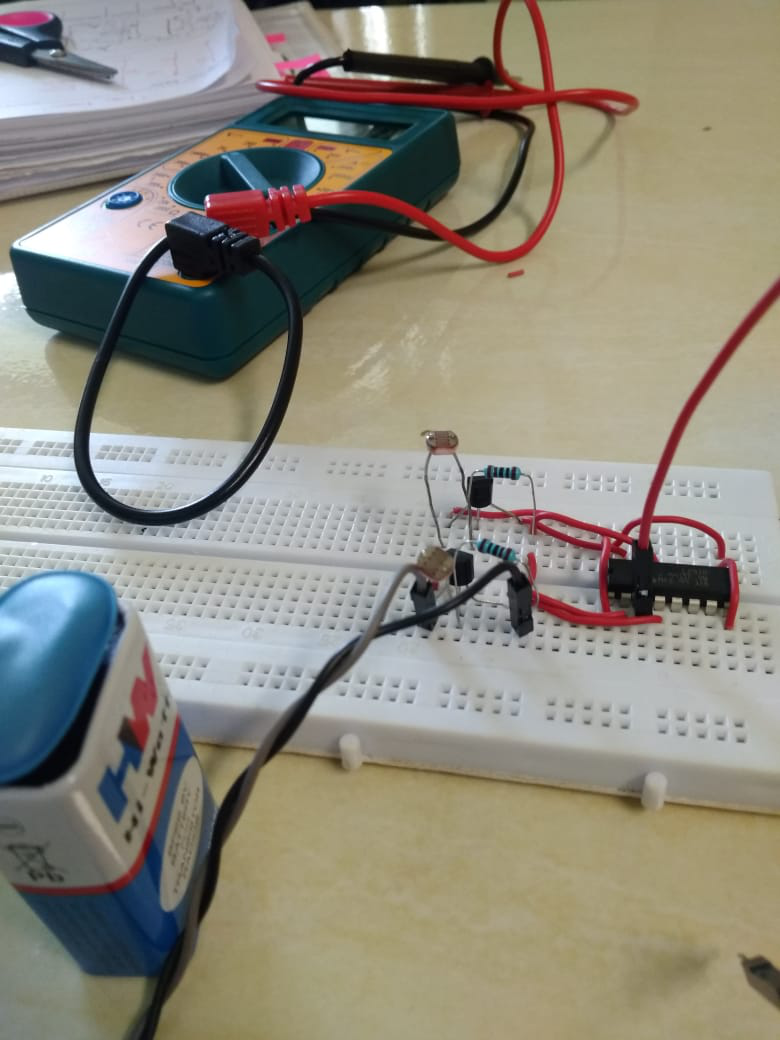
\includegraphics[width=6cm, height=12cm]{g1.png}
\end{center}
\paragraph{ }
\begin{center}
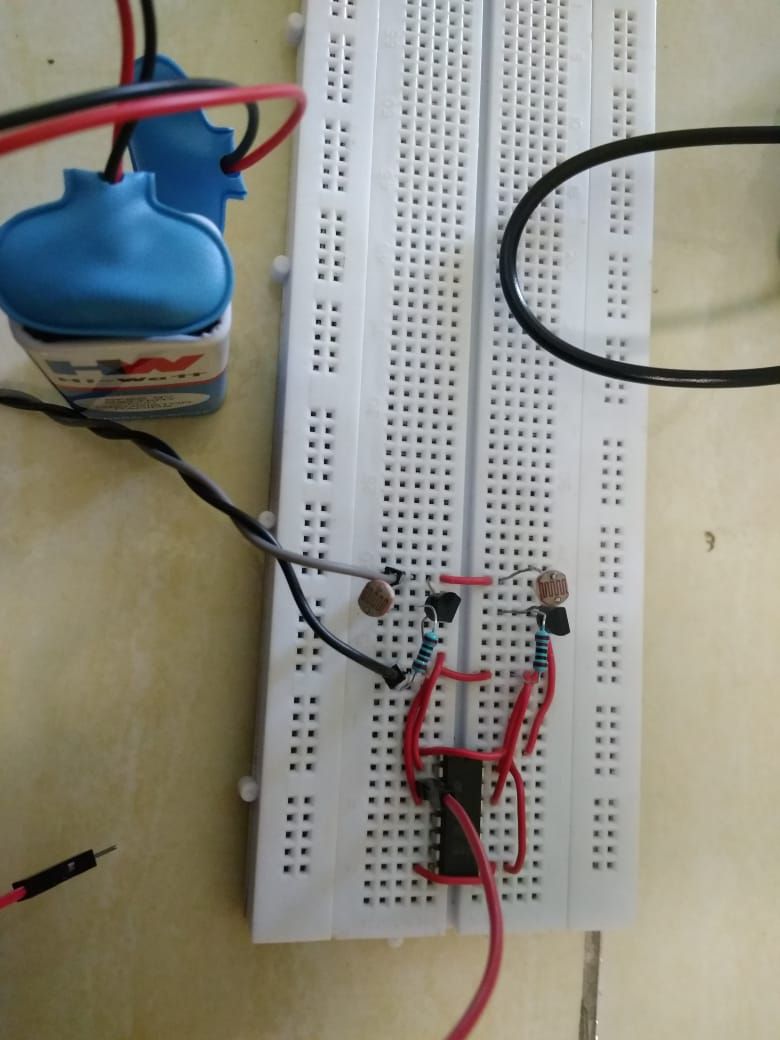
\includegraphics[width=6cm, height=12cm]{g2.png}
\end{center}
\end{figure}
\vspace{2cm}

\end{document} %Penulisan Laporan Berakhir
